%%%%%%%%%%%%%%%%%%%%%%%%%%%%%%%%%%%%%%%%%%%%%%%%%%%%%%%%%%%%%%%%%%%%%%%
%
%  A small sample UNSW Honours Thesis file.
%  Any questions to Ian Doust i.doust@unsw.edu.au
%
% Edited CSG 11.9.2015, use some of Gery's ideas for front matter; add a conclusion chapter.
%%%%%%%%%%%%%%%%%%%%%%%%%%%%%%%%%%%%%%%%%%%%%%%%%%%%%%%%%%%%%%%%%%%%%%%
%
%  The first part pulls in a UNSW Thesis class file.  This one is
%  slightly nonstandard and has been set up to do a couple of
%  things automatically
%
 
\documentclass[honours,12pt]{unswthesis}
\linespread{1}
\usepackage{amsfonts}
\usepackage{amssymb}
\usepackage{amsthm}
\usepackage{latexsym,amsmath}
\usepackage{mathtools}
\usepackage{graphicx}
\graphicspath{{/Users/odenpetersen/Documents/Honours/order-book-hawkes/images}}
\usepackage{afterpage}
\usepackage{xcolor}
\usepackage{tikz}
\usepackage[parfill]{parskip}


%%%%%%%%%%%%%%%%%%%%%%%%%%%%%%%%%%%%%%%%%%%%%%%%%%%%%%%%%%%%%%%%%
%
%  The following are some simple LaTeX macros to give some
%  commonly used letters in funny fonts. You may need more or less of
%  these
%
\newcommand{\R}{\mathbb{R}}
\newcommand{\Q}{\mathbb{Q}}
\newcommand{\C}{\mathbb{C}}
\newcommand{\N}{\mathbb{N}}
\newcommand{\F}{\mathbb{F}}
\newcommand{\PP}{\mathbb{P}}
\newcommand{\T}{\mathbb{T}}
\newcommand{\Z}{\mathbb{Z}}
\newcommand{\B}{\mathfrak{B}}
\newcommand{\BB}{\mathcal{B}}
\newcommand{\M}{\mathfrak{M}}
\newcommand{\X}{\mathfrak{X}}
\newcommand{\Y}{\mathfrak{Y}}
\newcommand{\CC}{\mathcal{C}}
\newcommand{\E}{\mathbb{E}}
\newcommand{\cP}{\mathcal{P}}
\newcommand{\cS}{\mathcal{S}}
\newcommand{\A}{\mathcal{A}}
\newcommand{\ZZ}{\mathcal{Z}}
%%%%%%%%%%%%%%%%%%%%%%%%%%%%%%%%%%%%%%%%%%%%%%%%%%%%%%%%%%%%%%%%%%%%%
%
% The following are much more esoteric commands that I have left in
% so that this file still processes. Use or delete as you see fit
%
\newcommand{\bv}[1]{\mbox{BV($#1$)}}
\newcommand{\comb}[2]{\left(\!\!\!\begin{array}{c}#1\\#2\end{array}\!\!\!\right)
}
\newcommand{\Lat}{{\rm Lat}}
\newcommand{\var}{\mathop{\rm var}}
\newcommand{\Pt}{{\mathcal P}}
\def\tr(#1){{\rm trace}(#1)}
\def\Exp(#1){{\mathbb E}(#1)}
\def\Exps(#1){{\mathbb E}\sparen(#1)}
\newcommand{\floor}[1]{\left\lfloor #1 \right\rfloor}
\newcommand{\ceil}[1]{\left\lceil #1 \right\rceil}
\newcommand{\hatt}[1]{\widehat #1}
\newcommand{\modeq}[3]{#1 \equiv #2 \,(\text{mod}\, #3)}
\newcommand{\rmod}{\,\mathrm{mod}\,}
\newcommand{\p}{\hphantom{+}}
\newcommand{\vect}[1]{\mbox{\boldmath $ #1 $}}
\newcommand{\reff}[2]{\ref{#1}.\ref{#2}}
\newcommand{\psum}[2]{\sum_{#1}^{#2}\!\!\!'\,\,}
\newcommand{\bin}[2]{\left( \begin{array}{@{}c@{}}
				#1 \\ #2
			\end{array}\right)	}
%
%  Macros - some of these are in plain TeX (gasp!)
%
\newcommand{\be}{($\beta$)}
\newcommand{\eqp}{\mathrel{{=}_p}}
\newcommand{\ltp}{\mathrel{{\prec}_p}}
\newcommand{\lep}{\mathrel{{\preceq}_p}}
\def\brack#1{\left \{ #1 \right \}}
\def\bul{$\bullet$\ }
\def\cl{{\rm cl}}
\let\del=\partial
\def\enditem{\par\smallskip\noindent}
\def\implies{\Rightarrow}
\def\inpr#1,#2{\t \hbox{\langle #1 , #2 \rangle} \t}
\def\ip<#1,#2>{\langle #1,#2 \rangle}
\def\lp{\ell^p}
\def\maxb#1{\max \brack{#1}}
\def\minb#1{\min \brack{#1}}
\def\mod#1{\left \vert #1 \right \vert}
\def\norm#1{\left \Vert #1 \right \Vert}
\def\paren(#1){\left( #1 \right)}
\def\qed{\hfill \hbox{$\Box$} \smallskip}
\def\sbrack#1{\Bigl \{ #1 \Bigr \} }
\def\ssbrack#1{ \{ #1 \} }
\def\smod#1{\Bigl \vert #1 \Bigr \vert}
\def\smmod#1{\bigl \vert #1 \bigr \vert}
\def\ssmod#1{\vert #1 \vert}
\def\sspmod#1{\vert\, #1 \, \vert}
\def\snorm#1{\Bigl \Vert #1 \Bigr \Vert}
\def\ssnorm#1{\Vert #1 \Vert}
\def\sparen(#1){\Bigl ( #1 \Bigr )}

\newcommand\blankpage{%
    \null
    \thispagestyle{empty}%
    \addtocounter{page}{-1}%
    \newpage}

%%%%%%%%%%%%%%%%%%%%%%%%%%%%%%%%%%%%%%%%%%%%%%%%%%%%%%%%%%%%%%
%
% These environments allow you to get nice numbered headings
%  for your Theorems, Definitions etc.  
%
%  Environments
%
%%%%%%%%%%%%%%%%%%%%%%%%%%%%%%%

\newtheorem{theorem}{Theorem}[section]
\newtheorem{lemma}[theorem]{Lemma}
\newtheorem{proposition}[theorem]{Proposition}
\newtheorem{corollary}[theorem]{Corollary}
\newtheorem{conjecture}[theorem]{Conjecture}
\newtheorem{definition}[theorem]{Definition}
\newtheorem{example}[theorem]{Example}
\newtheorem{remark}[theorem]{Remark}
\newtheorem{question}[theorem]{Question}
\newtheorem{notation}[theorem]{Notation}
\numberwithin{equation}{section}

%%%%%%%%%%%%%%%%%%%%%%%%%%%%%%%%%%%%%%%%%%%%%%%%%%%%%%%%%%%%%%%%%%
%
%  If you've got some funny special words that LaTeX might not
% hyphenate properly, you can give it a helping hand:
%
\hyphenation{Mar-cin-kie-wicz Rade-macher}

%%%%%%%%%%%%%%%%%%%%%%%%%%%%%%%%%%%%%%%%%%%%%%%%%%%%%%%%%%%%%%%%%%
% 
% OK...Now we get to some actual input.  The first part sets up
% the title etc that will appear on the front page
%
%%%%%%%%%%%%%%%%%%%%%%%%%%%%%%%%%%%%%%%%%%%%%%%%%%%%%%%%%%%%%%%%%

\setlength{\parindent}{0}
\setlength{\parskip}{2}



\title{Point Process Modelling of a Limit Order Book}

\authornameonly{Oden Petersen}

\author{\Authornameonly\\{\bigskip}Supervisor: Dr. Tom Stindl}

\copyrightfalse
\figurespagefalse
\tablespagefalse

%%%%%%%%%%%%%%%%%%%%%%%%%%%%%%%%%%%%%%%%%%%%%%%%%%%%%%%%%%%%%%%%%
%
%  And now the document begins
%  The \beforepreface and \afterpreface commands puts the
%  contents page etc in
%
%%%%%%%%%%%%%%%%%%%%%%%%%%%%%%%%%%%%%%%%%%%%%%%%%%%%%%%%%%%%%%%%%%

\begin{document}

\beforepreface

\afterpage{\blankpage}

% plagiarism

\prefacesection{Plagiarism statement}

\vskip 10pc \noindent I declare that this thesis is my
own work, except where acknowledged, and has not been submitted for
academic credit elsewhere. 

\vskip 2pc  \noindent I acknowledge that the assessor of this
thesis may, for the purpose of assessing it:
\begin{itemize}
\item Reproduce it and provide a copy to another member of the University; and/or,
\item Communicate a copy of it to a plagiarism checking service (which may then retain a copy of it on its database for the purpose of future plagiarism checking).
\end{itemize}

\vskip 2pc \noindent I certify that I have read and understood the University Rules in
respect of Student Academic Misconduct, and am aware of any potential plagiarism penalties which may 
apply.\vspace{24pt}

\vskip 2pc \noindent By signing 
this declaration I am
agreeing to the statements and conditions above.
\vskip 2pc \noindent
Signed: \rule{7cm}{0.25pt} \hfill Date: \rule{4cm}{0.25pt} \newline
\vskip 1pc

\afterpage{\blankpage}

% Acknowledgements are optional


\prefacesection{Acknowledgements}

\afterpage{\blankpage}

% Abstract

\prefacesection{Abstract}

This is the abstract
\afterpage{\blankpage}


\afterpreface

\afterpage{\blankpage}

\chapter{Introduction}\label{s-intro}

On a single day in 2023, the US stock market saw an average of around \$500 billion dollars worth of shares traded on various exchanges and other venues, exceeding the annual GDP of a typical European country \cite{FINRA2024}. Modern securities markets facilitate the exchange of shares and other financial assets at extremely high frequency, as a result of aggressive investment in specialised networking hardware, custom-made computer architectures, and high-throughput machine learning systems. In facilitating capital flows for the global economy, financial markets have at the same time managed to claim an increasing fraction of resources and attention, with economic consequences that are not yet fully understood \cite{Palley2007}.

Despite many mysteries and open questions about the origins and dynamics of market phenomena, the financial sector itself has readily adapted to the increasing scale and complexity of the markets in which it operates. The practical design of exchange rules and trading systems has in large part been an empirical endeavour on the part of market participants, operators, and regulators. Many phenomena have been observed to emerge in an apparently decentralised fashion from the application of exploitative heuristics and predictive algorithms that interact with exchanges and aggregate to produce desirable outcomes. While users of trading strategies aim to maintain acceptable risk levels while generating profits over the long term, market operators and regulators are tasked with the design of incentive mechanisms that exploit this self-interested behaviour to improve market outcomes, including reduced transaction costs, fast and accurate incorporation of external information (such as economic news or earnings reports), and adherence to various concepts of fairness, propriety, and legality.

In this thesis, I describe and extend prior work from the empirical market microstructure literature, making extensive use of the state-dependent Hawkes process model for event arrivals. I begin with a conceptual overview of the trading mechanism, and formalise the mathematical tools that will be used to construct and describe variations on the basic Hawkes process model. I continue with a summary of existing literature on point processes as applied to market data, including both mathematical foundations and empirical findings. Next, I explore techniques to reduce the computational burden of parametric inference for point processes on large datasets. Finally, empirical applications and findings are discussed, including applications of generative modeling to a variety of open problems in market microstructure.


\section{Limit Order Books}
Intraday trading allows participants to respond to exogenous news and endogenous market events in a manner that maintains acceptable levels of risk and generates profits over the long term. This activity has a significant influence on the formation of market prices and plays a key role in reducing transaction costs while increasing the speed at which large institutions can control their exposure to various financial risks and opportunities.

Securities exchanges facilitate automated matching of buyers and sellers at prices favourable to both. Understanding the dynamics of this exchange process at a high degree of resolution can provide insights into the design of automated \textit{matching engines} that produce desirable market behaviour, as well as insights into the design of \textit{trading strategies} that exploit the dynamics of the exchange process to generate profits.

A matching engine is tasked with receiving and acting on various messages from market participants indicating their intent to buy or sell a particular security with particular conditions. As a result of this process, trades may be formed that match buyers and sellers at a mutually agreeable price and quantity. Trade reports are broadcast to relevant participants and may be used for the purposes of risk management and forecasting, as well as for the ultimate transfer of the assets that have been traded (which often occurs after trading hours).

\bigskip

A typical matching engine permits two kinds of incoming messages, known as \textit{order insertion} and \textit{order cancellation}, and maintains an internal state consisting of a single data structure, known as a \textit{limit order book}.

\medskip

An order insertion message indicates a participant's willingness to buy (or sell) some quantity of a particular asset at or below (respectively, above) a particular price, and results in the addition of an \textit{order} to the limit order book $\mathcal{L}$.

Conversely, an order cancellation message results in the removal of a particular order from the limit order book, either in part (by reducing the remaining volume associated with the order) or in full (by removing the order entirely from the book). \textcolor{red}{It might be good to include a statistic about roughly how large cancellation rates are, to highlight the importance of this message type.}

Formally, a limit order book can be defined as a set of tuples (``orders'') of the form
$$(\text{side},\text{price},\text{time},\text{size}) = (s,p,t,q)\in \{-1,1\}\times P\times T\times Q.$$

Each published order represents an intention to buy (or sell) some quantity of an asset at a maximum (respectively, minimum) price, as illustrated in figure \ref{fig:limitorder}.

\begin{figure}[h]
	$$\left(\underbrace{-1}_{\fontsize{8}{8}\begin{matrix} \text{+1 for a buy order}\\ \text{-1 for a sell order}\end{matrix}}\fontsize{12}{8},\underbrace{84.1}_{\fontsize{8}{8}\begin{matrix}\text{The least favourable price}\\\text{(maximum for buy,}\\\text{minimum for sell)}\\\text{at which the order can trade}\end{matrix}}\fontsize{12}{8},\underbrace{9:52}_{\fontsize{8}{8}\begin{matrix}\text{The time at which the}\\\text{order was first published}\end{matrix}}\fontsize{12}{8},\underbrace{2}_{\fontsize{8}{8}\begin{matrix}\text{The maximum quantity}\\\text{of the product that will}\\\text{be traded with this order}\end{matrix}}\right)$$
	\caption{Components of an example limit order}
	\label{fig:limitorder}
\end{figure}

\newpage
\section{The Matching Algorithm}
\subsection{The Bid and Ask}
When an order insertion message is received, the exchange will attempt to form trades with the existing orders in the book such that as much volume as possible is matched. Any volume that cannot be matched will be added to the orders already in the book.

As a result of this matching, the total volume posted to the book may be depleted over time, even in the absence of cancellations. Any time a buy order has a price equal to or greater than that of a sell order, volume will be matched and a trade will occur. Consequently, the most competitive buy price (known as the \textit{bid}) will always be less than the most competitive sell price (known as the \textit{ask}), i.e.
	$$\text{bid}_\mathcal{L} = \max_{\left\{p : (1,p,t,q)\in\mathcal{L}\right\}} p \leq \min_{\left\{p : (-1,p,t,q)\in\mathcal{L}\right\}} p = \text{ask}_\mathcal{L}.$$

An excessively high bid price will be depleted by traders seeking to sell the product at a premium to its true value. Conversely, an excessively low ask price will be pushed up by participants hoping to buy at a discount. It is therefore common to regard the bid and ask as lower and upper bounds respectively on the consensus fair price of the product.

Motivated by this, the \textit{midprice} is a naive point estimate for the consensus fair price, defined by
	$$\text{mid}_\mathcal{L} = \frac{1}{2}\left(\text{bid}_\mathcal{L} + \text{ask}_\mathcal{L}\right).$$
Many other proxies for the consensus fair price exist, and it is common to use these as prediction targets in the construction of trading signals. \textcolor{red}{I might discuss them later}

\begin{figure}[h]
\begin{tikzpicture}
\draw[gray,thick] (0,3.5) -- (0,-3.5);

\draw[gray,thick] (-5,3) -- (0,3);
\draw[gray,thick] (-2,3) -- (-2,2);
\filldraw[black] (-1,2.5) node[opacity=0.8,fill=white,rounded corners=2pt,inner sep=1pt,rotate=15]{(-1,84.3,9:16,2)};
\draw[gray,thick] (-5,3) -- (-5,2);
\filldraw[black] (-3.5,2.5) node[opacity=0.8,fill=white,rounded corners=2pt,inner sep=1pt,rotate=15]{(-1,84.3,9:24,3)};

\draw[gray,thick] (-4,2) -- (0,2);
\draw[gray,thick] (-1,2) -- (-1,1);
\filldraw[black] (-0.5,1.5) node[opacity=0.8,fill=white,rounded corners=2pt,inner sep=1pt,rotate=15]{(-1,84.2,9:10,1)};

\draw[gray,thick] (-5,1) -- (0,1);
\draw[gray,thick] (-3,1) -- (-3,0);
\filldraw[black] (-1.5,0.5) node[opacity=0.8,fill=white,rounded corners=2pt,inner sep=1pt,rotate=15]{(-1,84.1,9:26,3)};
\draw[gray,thick] (-5,1) -- (-5,0);
\filldraw[black] (-4,0.5) node[opacity=0.8,fill=white,rounded corners=2pt,inner sep=1pt,rotate=15]{(-1,84.1,9:52,2)};

\draw[gray,thick] (-5,0) -- (0,0);

\draw[gray,thick] (6,-1) -- (0,-1);
\draw[gray,thick] (3,-1) -- (3,-2);
\filldraw[black] (1.5,-1.5) node[opacity=0.8,fill=white,rounded corners=2pt,inner sep=1pt,rotate=15]{(1,83.9,9:19,3)};
\draw[gray,thick] (5,-1) -- (5,-2);
\filldraw[black] (4,-1.5) node[opacity=0.8,fill=white,rounded corners=2pt,inner sep=1pt,rotate=15]{(1,83.9,9:34,2)};
\draw[gray,thick] (6,-1) -- (6,-2);
\filldraw[black] (5.5,-1.5) node[opacity=0.8,fill=white,rounded corners=2pt,inner sep=1pt,rotate=15]{(1,83.9,9:39,1)};

\draw[gray,thick] (6,-2) -- (0,-2);
\draw[gray,thick] (2,-2) -- (2,-3);
\filldraw[black] (1,-2.5) node[opacity=0.8,fill=white,rounded corners=2pt,inner sep=1pt,rotate=15]{(1,83.8,9:32,2)};
\draw[gray,thick] (4,-2) -- (4,-3);
\filldraw[black] (3,-2.5) node[opacity=0.8,fill=white,rounded corners=2pt,inner sep=1pt,rotate=15]{(1,83.8,9:48,2)};

\draw[gray,thick] (4,-3) -- (0,-3);

\filldraw[black] (0,0.5) circle (2pt) node[anchor=west]{ask};
\filldraw[black] (0,-0.5) circle (2pt) node[anchor=west]{mid};
\filldraw[black] (0,-1.5) circle (2pt) node[anchor=east]{bid};
\end{tikzpicture}
\caption{An example order book, arranged by order price and time}
\end{figure}

\subsection{Liquidity}
At any point in time, the contents of the limit order book represent trading opportunities presented to all market participants. The abundance of these opportunities, also known as \textit{liquidity}, represents a positive externality insofar as it allows impatient traders (\textit{liquidity takers}) to buy or sell products precisely under those circumstances where it is favourable to them. Conversely, order publishers (\textit{liquidity providers}) must adhere to the terms of trades formed against a posted order, regardless of whether it is in their interests.

One common measure for market liquidity is the \textit{bid-ask spread}, defined as
	$$\text{spread}_\mathcal{L} = \text{ask}_\mathcal{L} - \text{bid}_\mathcal{L}.$$
Notably, if $\text{mid}_\mathcal{L}$ is taken to represent the fair value of the product, the \textit{half-spread}, i.e. $\frac{1}{2}\text{spread}_\mathcal{L}$, represents the premium paid to liquidity providers by participants trading against the posted bid or ask. There are many other components and measures of liquidity \textcolor{red}{which I may discuss later}.

\subsection{Price-Time Priority}

\textcolor{red}{Explain}

\section{Queueing Models of the Order Book}

Queue depletions are related to price changes \cite{BouchaudEtAl}

Evolution of the limit order book over time $\to$ motivate the emphasis on modeling arrival times

Price evolution as a jump process (what is a jump process)
``Swishchuk and Huffman (2020) construct a compound Hawkes process'' modeling price changes with a jump process where jump sizes are a markov chain. Jump process is controlled by one-dimensional point process.
``Coinciding with the first preprint version of the present paper, Wu et al. (2019) develop a queue-reactive Hawkes process based on (2.4). In their model, X is endogenous and carries information about queue lengths in the LOB, while the multi-dimensional counting process driven by the intensity (2.4) models events pertaining to these queues. Wu et al. (2019) estimate their model on German bond (Bund) and index (DAX) futures LOB data.''
``Subsequently, Mounjid et al. (2019) generalise the queue-reactive Hawkes process to a more general point process framework that allows for non-linearity and quadratic Hawkes structure.  Mounjid et al. (2019) additionally establish ergodicity for the model and also derive functional limit theorems for its long-term behaviour. They apply the model to evaluate and rank equities market makers on Euronext Paris.''

Importance of arrival time modeling

\texttt{https://www.amazon.com/Point-Processes-Queues-Martingale-Statistics/dp/0387905367}

\section{Overview of Point Processes}
With the goal of modelling the arrival time process, I will now provide an introductory overview of point processes. In the next section, I will highlight some key variants described in existing literature that are relevant to order book modeling.

This section will make extensive use of theoretical concepts described in the appendix \textcolor{red}{Make sure to update this if there ends up being more than one appendix}. For an overview of measure theory, probability spaces, and stochastic processes, please refer to the relevant sections.

\subsection{Definition}
Given a probability space $(\Omega,\Sigma,\mathbb P)$, and a measurable space $(T,\Sigma_T)$ representing times, a point process is any increasing sequence of random times $$\mathcal T : \Omega\to T^\mathbb{N},$$
meaning that $\mathcal{T}(\omega)_n$ is increasing in $n$ for any $\omega\in\Omega$.

Concretely, $T$ may be chosen to be $\mathbb{R}_{\geq 0}$, and equipped with the Borel $\sigma$-algebra $B\left(\mathbb{R}_{\geq 0}\right)$.

The times in the point process are often referred to as \textit{event times}, with the implication that the sequence represents the times at which some event of interest occurs (for instance, the arrival of messages sent to a matching engine).

{\noindent}For any point process, there exists a corresponding càdlàg stochastic process $N_{\mathcal T}:T\times\Omega\to\mathbb{N}$ known as the \textit{counting process}, that gives the number of events having occurred before or at a given time. This is defined as
$$N_{\mathcal T}(t,\omega) = \vert \{i\in\mathbb N \vert \mathcal{T}(\omega)_i \leq t\} \vert.$$

\textcolor{red}{Overlay barcode plot for trade times with corresponding counting process}

All \textcolor{red}{(or perhaps many)} of the point processes considered in this thesis will additionally be adapted with respect to some filtration $\mathcal F$ indexed by $T$. \textcolor{red}{In what sense?}

Furthermore, I will only consider \textit{nonexplosive point processes}, defined as those point processes $\mathcal{T}$ for which
$$\lim_{n\to\infty}\mathcal{T}(\omega)_n=\infty, \mathbb{P}\text{-a.s.}$$

For any bounded interval of time $(t_{\min},t_{\max})$, a nonexplosive point process will almost surely contain only a finite set of times in that interval, i.e.
$$(t_{\min},t_{\max}) \cap \mathcal{T}(\omega) \text{ finite},\quad\mathbb{P}\text{-a.s.}$$

\subsection{The Counting Measure}
For any $\omega\in\Omega$, we can define the \textit{counting measure} $\Lambda_\omega$ of the point process as
$$\Lambda_\omega : \Sigma_T \to \mathbb{N}$$
$$\Lambda_\omega(S) \coloneq \left\vert S\cap \mathcal{T}(\omega)\right\vert.$$

For any finite or countable collection of disjoint sets $A_n\in\Sigma$, we have
$$\Lambda_\omega\left(\bigcup_n A_n\right) = \left\vert \bigcup_n \left(A_n\cap\mathcal{T}(\omega)\right)\right\vert.$$
Is this a measure on $(T,\Sigma_T)$? Since subsets of disjoint sets are also disjoint, the terms in the union on the right-hand side will be disjoint, and so
$$\Lambda_\omega\left(\bigcup_n A_n\right) = \sum_n\left\vert A_n\cap \mathcal{T}(\omega)\right\vert = \sum_n \Lambda_\omega(A_n).$$
So this is indeed a measure.

\subsection{The Expectation Measure}
Taking the expectation of the counting measure with respect to some measure $\mathbb{P}$ on a measurable space $(\Omega,\Sigma)$ gives the \textit{expectation measure},
$$\Lambda_\mathbb{P}(S)\coloneq \mathbb{E}_\mathbb{P}\left[\Lambda_\omega(S)\right] = \int_\Omega \Lambda_\omega(S)d\mathbb{P}(\omega).$$

Is this a measure on $(T,\Sigma_T)$? Since $\Lambda_\omega(S)$ is a non-negative function of $\omega$, it follows that $$\Lambda_{\mathbb{P}} : \Sigma_T \to \mathbb{R}_{\geq 0}\cap\{\infty\}.$$ Furthermore, for any finite or countable sequence of $A_n\in B(\mathbb{R})$, we have $$\Lambda_\mathbb{P}\left(\bigcup_n A_n\right) = \int_\Omega \Lambda_\omega\left(\bigcup_n A_n\right)d\mathbb{P}(\omega) = \int_\Omega \sum_n \Lambda_\omega(A_n) d\mathbb{P}(\omega),$$
by the countable additivity of $\Lambda_\omega$.

To handle the sum inside the integral, we can write each term as a sum of indicator functions:
$$\Lambda_\omega(A_n) = \left\vert A_n\cap \mathcal{T}(\omega)\right\vert = \sum_i 1_{A_n}\left(\mathcal{T}(\omega)_i\right).$$
Then, since $A_n$ are measurable sets, the indicator functions are each measurable functions of $\omega$. Because finite sums and pointwise limits of measurable functions are measurable, we have that $\Lambda_\omega(A_n)$ is measurable.  Finally, since each term in the sum over $n$ is a nonnegative measurable function, the integral commutes with the sum, and hence $\Lambda_\mathbb{P}$ is countably additive. Therefore the expectation measure is also a valid measure.

\subsection{Intensity of a Point Process}
For a point process $\mathcal{T}$, the counting measure of a half-open interval $(t,t+\epsilon]$ can be written in terms of the counting process $N_\mathcal{T}$ in the form
$$\Lambda_\omega\left((t,t+\epsilon]\right) = N_\mathcal{T}(t+\epsilon,\omega) - N_\mathcal{T}(t,\omega).$$
Integrating out $\omega$ with respect to $\mathbb{P}$ then gives us the identity
$$\Lambda_\mathbb{P}\left((t,t+\epsilon]\right) = \mathbb{E}_\mathbb{P}\left[N_\mathcal{T}(t+\epsilon)\right] - \mathbb{E}_\mathbb{P}\left[N_\mathcal{T}(t)\right],$$
allowing us to write the expectation measure in terms of a finite difference of the first moment of $N_\mathcal{T}$.

If $\mathbb{E}_\mathbb{P}\left[N_\mathcal{T}(t)\right]$ is right-differentiable at $t$, we can further say that
$$\lim_{\epsilon\to0}\frac{\Lambda_\mathbb{P}\left((t,t+\epsilon]\right)}{\epsilon} = \lim_{\epsilon\to0}\frac{\mathbb{E}_\mathbb{P}\left[N_\mathcal{T}(t+\epsilon)\right] - \mathbb{E}_\mathbb{P}\left[N_\mathcal{T}(t)\right]}{\epsilon} = \frac{d\mathbb{E}_\mathbb{P}\left[N_\mathcal{T}(t)\right]}{dt}$$
for sufficiently small $\epsilon$, where the last term is the right-derivative. For brevity, I will write
$$\lambda_{\mathbb{P}}(t) \coloneq \frac{d\mathbb{E}_\mathbb{P}\left[N_\mathcal{T}(t)\right]}{dt}.$$

Assuming further that $\mathbb{E}_\mathbb{P}\left[N_\mathcal{T}(t)\right]$ is differentiable on some open interval $(t,t+\epsilon')$, \textcolor{red}{Prove this is Radon-Nikodym derivative of $\Lambda_\mathbb{P}$ in the open interval}

It then follows from the fundamental theorem of calculus that
$$\int_t^{t+\epsilon} \lambda_{\mathbb{P}}(s)ds = \lambda_{\mathbb{P}}(t)\cdot\epsilon + o(\epsilon),\quad \epsilon\to 0.$$

So \textcolor{red}{since $\lambda_\mathbb{P}$ is a radon-nikodym derivative} we can write \textcolor{red}{Why?}
$$\Lambda_{\mathbb{P}}\left((t,t+\epsilon]\right)=\lambda_{\mathbb{P}}(t)\cdot\epsilon+o(\epsilon),\quad \epsilon\to 0$$
Therefore the expected number of events occurring in a small interval $(t,t+\epsilon]$ is approximately proportional to its length.

It is common to refer to $\lambda_{\mathbb{P}}(t)$ as the \textit{arrival rate} of the point process at $t$, since it represents the expected number of events occurring per unit time.

If we instead take the expectations above conditioned on $\mathcal{F}_t$, we can define a stochastic process
$$\lambda(t,\omega) \coloneq \lambda_{\mathbb{P}\vert\mathcal{F}_t}(t,\omega),$$
known as the \textit{intensity} of the point process. This represents our best estimate of the number of events that will arrive in the next $\epsilon$ units of time, for very small $\epsilon$, based on all the information contained in the filtration up to $t$.

\textcolor{red}{Existence and uniqueness shown in https://projecteuclid.org/journals/annals-of-probability/volume-24/issue-3/Stability-of-nonlinear-Hawkes-processes/10.1214/aop/1065725193.full under restrictions on the kernel}

\subsection{Residuals}
\textcolor{red}{Define residuals, explain why they're exponentially distributed}

\subsection{Marked and Multivariate Point Processes}

A point process \mathcal{T} may be \textit{marked}, in which case it is associated with one or more random sequences of marks $$\mathcal{X}:\Omega\to X^\mathbb{N},$$
drawn from a set $X$, that represent additional information about each event. These may be adapted to the filtration $\mathcal{F}$ \textcolor{red}{In what sense?}

A common special case of this is when $X$ is partitioned into a finite number of \textit{event types}, in which case we may refer to $\mathcal{T}$ as a \textit{multivariate point process}.

Each part $E$ of the partition then has an associated point process $$\mathcal{T}_E = \mathcal{T}_{\{n\in\mathbb{N} : \mathcal{X}_n\in E\}},$$ formed by the subsequence of times where the corresponding element of $\mathcal{X}$ is in $E$. These point processes will then have their own counting functions, intensities, and other characteristics. It is common to arrange these in vector form, with one entry for each event type.

On the other hand, given a collection of point processes adapted with respect to a common filtration, we can form a single marked point process by interleaving the sequences of event times. The counting process, counting measure, expectation measure, and intensity of the combined process will be the sum of those for the individual point processes.

\textcolor{red}{Barcode plot and counting process for buys and sells, and the combined process}

%Marked point processes have marks that are not independent of the point process itself. This is probably important to note. Continuous marks can also have this property; usually they won't affect the future behaviour of the point process though.


\section{Point Process Models of Book Updates}

\textcolor{red}{
For each extension:
- show some example realisations for various parameter choices: barcode and intensity plot
}


\subsection{Poisson Processes}
Probably the simplest modeling assumption we can make is to assume that the intensity of the process is a constant $\nu\in\mathbb{R}$.

A Poisson process is a point process for which the following two properties hold.
\begin{enumerate}
	\item For any finite collection of disjoint measurable sets $A_n\in\Sigma_T$, their counting measures $\Lambda_\omega(A_n)$ are independent random variables.
	\item For any measurable set $A\in\Sigma_T$, we have $$\Lambda_{\mathbb P}(A) = \nu \mu_{\mathrm{Lebesgue}}(A)\propto\mu_{\mathrm{Lebesgue}}(A).$$
\end{enumerate}
\textcolor{red}{Why is this the same as saying that the intensity is constant?}

In the multivariate case with $n$ event types, we have a vector $\nu\in\mathbb{R}_{>0}^n$ containing the constant intensities of each individual point process.

\textcolor{red}{This definition might require a reference.}

\textcolor{red}{Is there a proof of existence and nonexplosiveness?}

\textcolor{red}{Explain why the times between events are exponentially distributed. Can use the linearity of residuals to prove this succinctly, since residuals are exponentially distributed.}

\textcolor{red}{There is a link here to the sante fe order book model, described in the Bouchaud source, which is an example of the application of poisson arrivals.}

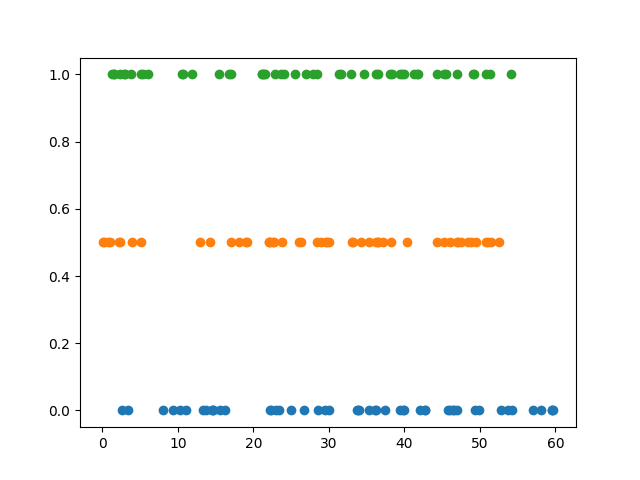
\includegraphics[width=0.75\textwidth]{poisson_sim.png}

\textcolor{red}{I think I should change this to be separate plots. Can show the intensity function for each; e.g. for inhomogenous it's the same for every realisation, but for hawkes process the intensity function is itself random.}

\subsection{Inhomogeneous Poisson Process}
An inhomogeneous Poisson process is a generalisation of the Poisson process for which the second condition is replaced by the weaker requirement that every measurable set $A\in\Sigma_T$ with finite Lebesgue measure $\mu_{\mathrm{Lebesgue}}(A)$ has a finite expectation measure. \textcolor{red}{Is this weaker version even needed, or is it sufficient to just drop the condition entirely?}

As a result, although the intensity $\lambda(t,\omega)$ is constant in $\omega$ (i.e. deterministic) \textcolor{red}{how do we know it is?}, it can vary as a function of $t$. This is useful for modeling deterministic seasonality in the point process, such as having more events near the start/end of each trading session or near known events such as news releases.

\textcolor{red}{Show U-shape from empirical data}
\textcolor{red}{Show U-shape from quadratic IPP}

\subsection{Autoregressive Point Processes}



i.e. Hawkes Processes
\textcolor{red}{Intuitively, self-excitation or self-inhibition; mutually exciting/inhibiting}

\textcolor{red}{Original hawkes process paper https://academic.oup.com/biomet/article-abstract/58/1/83/224809?redirectedFrom=fulltext}

immigration/birth interpretation
branching matrix \& complete data likelihood

Long-run mean $$\bar\lambda = \lim_{t\to\infty} \mathbb E\left[\lambda(t)\right]$$

$$\bar\lambda = \nu + \bar\lambda \int_0^\infty k(t)dt$$

Stability requires $\int_0^\infty k(t)dt < 1$. Not sure if sufficient condition.

Multidimensional:
$$\bar\lambda = \nu + K \bar\lambda$$
$$\bar\lambda = (I-K)^{-1}\nu$$
Requires $\vert\det K\vert < 1$ (why? and what about if there are directions orthogonal to $\nu$?)
\textcolor{red}{Define K}

According to \texttt{https://ieeexplore.ieee.org/document/7416001 https://arxiv.org/pdf/1401.0903}, hawkes processes are fully determined by the first two moments of the intensity function. Proof in the paper.


Special case of $\beta=0$ may be worth including in the final kernel. (Integrated point process?)


\subsection{State Dependence}
Vinovskaya proposes regime-switching independent of the point process
Moriaru-Patrichi and Pakkanen generalise this by coupling state transitions with the event sequence. They consider conditioning on only the state of the triggering event (their 2.3), as well as conditioning on both the state of the triggering event and the current state (their 4.2).
Moriaru-Patrichi and Pakkanen find that conditioning on the state of the order book improves the fit of the model. (How?)

``Cohen and Elliott (2013) introduce a one-dimensional Markov-modulated Hawkes process following (2.4), where X is an exogenous Markov process in a finite state space (exogenous in the sense that the counting process does not influence X).  The key feature of their work is that they assume X to be unobservable, leading them to derive a filtering procedure for the estimation of the current state of X.'' (hidden states)


The first of these:
	$$\tilde\lambda_{ex}(t)=\phi_e(X(t),x)\left(\nu_e+\sum_{e'\in\mathcal E,x'\in \mathcal X}\int_{[0,t)}k_{e',e}(t-s,x')d\tilde N_{e'x'}(s)\right), & t\geq 0, & e\in\mathcal E, & x\in\mathcal X.$$

The second:
	$$\tilde\lambda_{ex}(t)=\nu_{ex}+\sum_{e'\in\mathcal E,x'\in\mathcal X}\int_{[0,t)}k_{e'x'ex}(t-s)d\tilde N_{e'x'}(s), t\geq 0, e\in\mathcal E, x\in\mathcal X.$$


1. markov switching
2. linear state space model / kalman filter (we'll see if i get around to figuring out how to work this)

\subsection{Regression on marks}

Multiply the kernel by $\exp\left(X\cdot\beta\right)$ where $X$ is a vector of mark variables and $\beta$ are coefficients.
\textcolor{red}{transfer functions should be separable, see [6.25 Definition] in https://www.research-collection.ethz.ch/bitstream/handle/20.500.11850/151886/eth-1112-02.pdf}

\subsection{Adding structure to the event space}
For a finite number of event types (e.g. 10 book levels) this just corresponds to constraining the coefficient matrices.

For a continuous event space it is a bit more complicated


Another way to look at this is just having marks but the distribution of the marks is not constant - this works too. This approach is nice because it admits Kalman filtering. (Is it possible to mix Kalman filtering in event time, volume time, and wall time? Maybe better to just use wall time though.)

\subsection{Hidden Events}
\textcolor{red}{Seems relevant https://www.cambridge.org/core/journals/advances-in-applied-probability/article/abs/an-elementary-derivation-of-moments-of-hawkes-processes/79A7355542F08087C8AE828C664A3049}

\textcolor{red}{Hawkes Process Inference with Missing Data https://aaai.org/papers/12116-hawkes-process-inference-with-missing-data/ makes use of monte carlo EM algorithm https://www.jstor.org/stable/2290005?seq=1}

\textcolor{red}{Hawkes processes with hidden marks https://www.tandfonline.com/doi/full/10.1080/1351847X.2020.1820356?scroll=top&needAccess=true}

Meta-orders. Kernel is product of an ordinary kernel and an EMA on the meta-order hidden events. See model in \cite{BouchaudEtAl} 10.4.3.

Could also be used to correct for the quasi-EM approximation.

\section{the most general model}
\textcolor{red}{Here for ideas/reference but I dont think this section will be in the final report}
State-dependent multi-kernel multivariate hawkes process with increasing kernel components and possible inhibition.

Nonparametric estimate of nu, sim study for u-shaped true nu. Probably splines, maybe kde if its fast enough. Compare to quadratic regression

The marks evolve according to state-space model involving various model variables, but have no causal impact on the point process (though obviously there is state-dependence, and the state may include the marks).

The state might be generalised to a kalman-filter-ish model \cite{SmithBrown}

$$IRF_{e,e',k}(s,t) = \alpha_{e,e',k} e^{X(s)\cdot c_{e,e',k}}\exp\left(-\beta_{e,e',k}(t-s)\right)$$
$$\lambda_{e,e',k}(t,\omega) = \int_0^t IRF_{e,e',k}(s,t) d\Lambda_{e',\omega}(s)$$
$$\lambda_e(t,\omega) = \sum_{e'} \sum_k \lambda_{e,e',k}(t,\omega) + \text{spline intensity}(t)$$


\chapter{Estimation}%\label{something}

To enable analysis of empirical order book data, I will now explain the principles involved in parameter estimation for point process models.

\section{Empirical Counting Measure}
Define $\lambda_{e,(T,E)}(t)$ and $\Lambda_{e,(T,E)}(t)$ for fully observed point processes for $(T,E)$

\section{Maximum Likelihood Estimation}
Given a parametric family of marked point processes,
$$\{(\mathcal{T}_\theta,\mathcal{X}) : \theta\in\Theta\}$$


\textcolor{red}{Derive the likelihood function}

For a particular observation $(T,E)$, we have

$$\ell((T,E);\theta) = \sum_e \left(\int_0^T \log(\lambda_{e,\theta,(T,E)}(t))d\Lambda_{e,(T,E)}(t)-\int_0^T \lambda_{e,\theta,(T,E)}(t)dt\right)$$

\textcolor{red}{What is a likelihood function}


Clearly $\lambda_e$ must be positive at the event times.

At stationary points, loglikelihood has zero derivatives.

$$\frac{\partial \ell((T,E);\theta)}{\partial \theta} = \sum_{e}\left(\int_0^T \frac{\partial \lambda_{e,\theta,(T,E)}(t)}{\partial \theta}\cdot\frac{1}{\lambda_{e,\theta,(T,E)}(t)}d\Lambda_{e,(T,E)}(t) - \int_0^T \frac{\partial\lambda_{e,\theta,(T,E)}(t)}{\partial \theta}dt\right)$$

Explain why no explicit solution

Observe that if intensity is a sum of multiple kernels it separates into the EM form

Introduce the branching matrix

Motivate iterative methods: find an iteration whose fixed points are stationary points. Is there a way to show that this converges?

\section{EM}

\subsection{Information Theory and EM}
\textcolor{red}{Can cite original dempster paper? As well as the one that corrects the errors in that paper}

\subsection{EM for Hawkes Processes}
Branching matrix vs exo/endo classification. Usefulness for multikernel and other limitations of gradient based MLE.

\begin{align*}
	B_{e,e',k}(s,t)
	&= \frac{IRF_{e,e',k}(s,t)}{\lambda_{e}(t)} \\
\end{align*}
\begin{align*}
	\sum_{e'} \sum_{k} \int_0^t B_{e,e',k}(s,t)d\Lambda_{e',\omega}(s) = 1
\end{align*}

Branching matrix:
\begin{align*}
	B_{i,j,k} = \frac{IRF_{e_j,e_i,k}(t_i,t_j)}{\lambda_{e_j}(t_j)}
\end{align*}

- Visualisation of branching matrix. How does it evolve throughout the fitting procedure?
- Quasi EM approximation
- Closed form constant time M step
- Negative probabilities. Conditions for kernel nonnegativity? (Probably not tractable)
- Complex probabilities? For periodic/wavelet kernels

\subsection{Generalised Fixed Point Methods}
\textcolor{red}{Is it a contraction mapping?}

\subsection{Method of Scoring (Newton's Method)}

\section{Uncertainty quantification for MLE}
Asymptotic normality

Parametric Bootstrap

\section{Inference for the Mark Process}
Kalman filter? Ways to couple this with the point process? (Monte carlo EM?)

\section{Computational Concerns}
Sensor fusion for parallelisation

Momentum (analyse autocorrelation of parameter changes throughout the learning process)

Exploiting sparsity \cite{NickelLe}

\section{Bayesian Approach}
- Uncertainty quantification
- Less likely to get stuck in local optima
- Jeffreys prior: $\sqrt{\det \mathcal{I}}$

\section{Model Selection}

\textcolor{red}{Performance of information criteria for selection of Hawkes process models of financial data https://www.tandfonline.com/doi/full/10.1080/14697688.2017.1403140}

\chapter{Generative Sampling}
\section{Simulation Methods}
Immigration-birth interpretation \cite{MorariuPatrichiPakkanen}
(aka Watson-Galton models)

\textcolor{red}{Pseudocode}

Ogata thinning \bibitem{Ogata}

\textcolor{red}{Pseudocode}

\textcolor{red}{Do these have different time complexity? Memory complexity?}

\section{Simulation Study of Estimation Methods}
Convergence analysis for simple models (eg univariate)

\section{Impulse Response Function}
Causal analysis, price impact of orders.

What does inserting a single exogenous event do to the order book, price, etc? Are there analytical formulas for this?


\cite{AbergelJedidi} \cite{Toke} sources that use hawkes process models to simulate an order book for analysis purposes


\chapter{Application to KOSPI/SPY Data} %Maybe make this 2 different chapters
\textcolor{red}{Hawkes processes and their applications to finance: a review https://www.tandfonline.com/doi/full/10.1080/14697688.2017.1403131}
\textcolor{red}{https://www.tandfonline.com/journals/rejf20/collections/Hawkes-Processes-in-Finance}


\begin{itemize}
	\item Basic poisson model
	\item Univariate hawkes
	\item Multivariate hawkes - what are the event types?
	\item State-dependent hawkes - which state variables are relevant?
	\item Full model
	\item Replicate findings from \cite{MorariuPatrichiPakkanen}
	\item Hidden events (\& events on different exchanges) - either poisson distributed or more complex
	\item Modeling changes in the entire order book
	\item Market impact (are there any datasets on this? square-root law, other common findings. power law impact for hawkes processes is explicitly studied here \texttt{https://arxiv.org/pdf/1805.07134})
	\item Optimal execution - VWAP, TWAP, Almgren-Chriss
	\item Midprice change prediction/explanation - explicit formula or simulation?
	\item Realised volatility prediction
	\item Correlated products (with low beta, preferably - or see what is done in literature studies of correlated products)
	\item Options (if I can get data) - would give lots of (nonlinearly) correlated products. Can estimate the correlation between products at any point in time using factor loadings \& historical factor correlations. Here is one source: \texttt{https://www.nber.org/system/files/working_papers/w29369/w29369.pdf}. Options price impact: \texttt{https://arxiv.org/abs/1602.03043}
	\item Closed form for optimal execution of signals (including cross-impact)
	\item This paper arxiv.org/pdf/2401.11495 shows a functional limit theorem for hawkes processes behaving as integrated CIR processes. These are a popular volatility model so this makes sense!
\end{itemize}

$\texttt{https://quant.stackexchange.com/questions/59593/what-are-some-currently-open-problems-in-market-microstructure}$
\texttt{https://papers.ssrn.com/sol3/papers.cfm?abstract_id=4844711 Option Pricing Using Hawkes Process}
\texttt{https://quant.stackexchange.com/questions/4259/analyzing-tick-data}

\textcolor{red}{A slightly depressing jump model: intraday volatility pattern simulation https://www.tandfonline.com/doi/full/10.1080/14697688.2017.1403139}
\textcolor{red}{Implementation and evaluation of the Heston-Queue-Hawkes option pricing model https://uu.diva-portal.org/smash/get/diva2:1763609/FULLTEXT01.pdf}

\subsection{Clustering Ratio}
\textcolor{red}{Variance of interevent time divided by expectation. Bouchaud p 165. Should this section be elsewhere? Does this mean something for residuals too?}

Point process control \texttt{https://pages.stern.nyu.edu/~rcaldent/courses/B60.4308_files/Point-Process.pdf}

Two choices for handling inhomogeneity:
- Reparameterise to 'business time' in preprocessing, as recommended by \cite{BouchaudEtAl} in 9.3.1
- Splines/polynomials etc
- Could also combine both


Databento info:
CME:
ES
MES
OPRA:
SPX - Index options
SPY - Index ETF options
https://databento.medium.com/getting-futures-tick-sizes-and-notional-tick-values-in-python-with-databento-ba03cfded553

\chapter{Conclusion}\label{ccl}


This is the conclusion


\chapter{Appendix: Foundations of Probabilistic Models}
In order to describe precisely the various models explored in this thesis, it is necessary to introduce some key mathematical concepts that form the basis for model specifications and related derivations. In this appendix, I cover the basics of measure, probability, and stochastic processes.

\section{Measure Theory Fundamentals}
In order to formalise the concept of a stochastic process, it is necessary to introduce the concept of a measure space.

For any set $X$, we can construct the power set
$$\mathcal{P}(X) = \{S : S\subseteq X\}$$
which is a new set that contains as its elements every subset $S$ of $X$.

We say that a subset $\Sigma$ of $\mathcal{P}(X)$ is a  \textit{$\sigma$-algebra} on $X$ if and only if it satisfies the following three properties:
\begin{enumerate}
	\item Containment of the full space, i.e. $$X\in\Sigma.$$
	\item Closure under complements, i.e. $$\forall S \in \Sigma, X\backslash S\in\Sigma.$$
	\item Closure under countable union, i.e. $$\forall \{A_n\}_{n=0}^\infty\in\Sigma^{\mathbb{N}},\quad\bigcup_{n=0}^\infty A_n \in \Sigma.$$
\end{enumerate}
Elements of $\Sigma$ are known as \textit{measurable sets}. A common example of a $\sigma$-algebra is the Borel $\sigma$-algebra $B(X)$ of a topological space $X$ (e.g. $\mathbb{R}$), defined as the smallest $\sigma$-algebra such that every open set is measurable.

We then say that a \textit{measure} on $(X,\Sigma)$ is any function $\mu:\Sigma\to\mathbb{R}_{\geq 0}\cup\{\infty\}$ that is \textit{countably additive}, meaning that for any finite or countable sequence of disjoint sets $A_n\in\Sigma$, we have
$$\mu\left(\bigcup_n A_n\right) = \sum_n \mu(A_n).$$
Assuming that at least one set $S\in\Sigma$ has finite measure, we then have $$\mu(S)=\mu(S\cap\emptyset)=\mu(S)+\mu(\emptyset) \implies \mu(\emptyset)=0.$$
We refer to the combined triple $(X,\Sigma,\mu)$ as a \textit{measure space}.

Informally, a measure formalises intuitions about the size, mass, or significance of a set of points. For instance, a set $S\subseteq X$ with measure zero is known as a \textit{null set}, and a property that holds only for points in a null set is said to be true \textit{almost nowhere} in $X$. Conversely, a property that holds for every point except those in a null set is said to be true \textit{almost everywhere} (a.e.) in $X$. In this way, a measure quantifies how significant or negligible the exceptions to a heuristic principle may be.

Similarly, familiar concepts of \textit{length}, \textit{area} and \textit{volume} are all formalised by a family of translation-invariant measures on $\mathbb{R}^n$, known as the $n$-dimensional \textit{Lebesgue measures}.

The concept of a measure is foundational to the definition of the Lebesgue integral. Integration of a function $f$ over a measurable set $S$ with respect to a measure $\mu$ is written as
$$\int_{t\in S} f(t) d\mu(t),$$
while integration with respect to the Lebesgue measure will often be written simply as
$$\int_S f(t)dt.$$
I will not cover the definition of the Lebesgue measure or Lebesgue integral here, but they can be found in most textbooks on measure theory.

\section{Probability Spaces}
In the special case where $\mu(X)=1$, we refer to $\mu$ as a \textit{probability measure}, and to $X$ as a \textit{sample space}. Correspondingly, the term \textit{almost everywhere} is replaced with \textit{almost surely} (a.s.), indicating a property that holds on a set of points with probability measure one.

A function from one $\sigma$-algebra to another is called \textit{measurable} if and only if the preimage of any measurable set in the codomain is a measurable set in the domain. A measurable function whose domain is a sample space $\Omega$ equipped with a probability measure $\mathbb{P}$ is known as a \textit{random variable}.

Measurable sets in a sample space are often referred to as \textit{events}, and the measure of such a set is called the probability of the event. For instance, the set $S$ of points $\omega\in\Omega$ for which a random variable $X:\Omega\to\mathbb{R}$ satisfies a particular property $P:\mathbb{R}\to\{\mathrm{True},\mathrm{False}\}$ will have measure equal to the probability of that property being true.\footnote{The predicate $P$ must be measurable.}

A more general concept is \textit{expectation}. For a real-valued random variable $X:\Omega\to \mathbb{R}$, we define the expectation of $X$ with respect to $\mathbb{P}$ to be the linear functional
$$\mathbb{E}_{\mathbb{P}}[X(\omega)] \coloneq \int_{\omega\in\Omega} X(\omega)d\mathbb{P}(\omega).$$

For binary-valued random variables $X:\Omega\to\{0,1\}$, we have the identity
$$\mathbb{E}_\mathbb{P}[X(\omega)] = \mathbb{P}\left(\{\omega\in\Omega : X(\omega)=1\}\right).$$

\subsection{Conditionalisation}
By defining ``events" as $\Sigma$-measurable subsets of $\Omega$, we allow knowledge of an event to inform us about which possible values of the hidden $\omega$ could have produced the result we actually observe. In this way, the knowledge that $\omega$ has produced one observed event allows us to draw probabilistic conclusions about the occurrence of a different, related event. For instance, learning that a die has rolled an even number tells us that it cannot possibly have rolled a $3$, and makes the proposition that a $2$ has been rolled a more reasonable guess than otherwise.

In order to capture the relationships between events, and to make systematic inferences about hidden events from observed ones, it is necessary to describe mathematical rules for \textit{conditionalisation}.

Given two $\sigma$-algebras $\Sigma_1,\Sigma_2$ on $\omega$, we say that $\Sigma_1$ is a \textit{sub-$\sigma$-algebra} of $\Sigma_2$ if and only if $\Sigma_1\subseteq\Sigma_2$. In the case where $\Sigma_1\not=\Sigma_2$, $\Sigma_1$ is said to be \textit{coarser} than $\Sigma_2$, in the sense that $\Sigma_2$ contains events that cannot be expressed as $\Sigma_1$-measurable sets. Knowing which $\Sigma_2$-events the hidden $\omega$ falls under can therefore give us more information about the exact value of $\omega$.

One common example of a sub-$\sigma$-algebra arises by considering the set
$$\{X^{-1}(A) : A\in\mathbb{R}\}\subseteq\mathcal{P}(\Omega),$$
consisting of all the preimages of Borel-measurable sets under a random variable $X:\Omega\to\mathbb{R}$. This is known as the $\sigma$-algebra generated by $X$.

expectation conditional on sigma algebra
https://math.stackexchange.com/questions/2373097/condition-on-sigma-algebra
expectation conditional on an event


probability is expectation of indicator function (notation for indicator function is $1_A$)

random measure

What is independence
independence of RVs if and only if independence of generated sigma algebras

Conditional probability

\section{Density of a Measure}
\textcolor{red}{Absolute continuity: $\mu_1\ll\mu_2$ ($mu_1$ is dominated by $\mu_2$) if and only if $\mu_2(A)=0\implies\mu_1(A)=0$ for every measurable set $A$. Can also say that one measure is absolutely continuous wrt another on a subset of the measure space}
\textcolor{red}{Radon-Nikodym Theorem}

\section{Stochastic Process Fundamentals}
What is a filtration

What is a stochastic process

What is a realisation of a stochastic process

What is a cadlag \textcolor{red}{The order book is a cadlag over time. Also the counting process is a cadlag.}

\textcolor{red}{What is a martingale - do I need this?}




%%%%%%%%%%%%%%%%%%%%%%%%%%%%%%%%%%%%%%%%%%%%%%%%%%%%%%%%%%%%%%%%%%%%%%%%%%

\clearpage
\addcontentsline{toc}{chapter}{References}
\bibliographystyle{unswthesis}

\begin{thebibliography}{999}

\bibitem{Palley2007}
Palley, T. I.,
\textit{Financialization: What It Is and Why It Matters},
Working Paper No. 525, The Levy Economics Institute, December 2007.
Paper presented at the conference on “Finance-led Capitalism? Macroeconomic Effects of Changes in the Financial Sector,” sponsored by the Hans Boeckler Foundation, Berlin, Germany, October 26–27, 2007.
Available at: \url{https://www.levyinstitute.org/pubs/wp\_525.pdf}

\bibitem{BalakrishnanWainwrightYu}
Balakrishnan, S., Wainwright, M. J., and Yu, B.,
\textit{Statistical guarantees for the EM algorithm: From population to sample-based analysis},
\textit{The Annals of Statistics},
\textbf{45}(1) (2017), 77--120.
doi = {10.1214/16-AOS1435}
\textcolor{red}{various facts about EM algorithm in general, useful in particular because it shows the general principle that likelihood gradient = EM gradient. balakrishnan, wainwright, yu page 82 as cited at https://stats.stackexchange.com/questions/45652/what-is-the-difference-between-em-and-gradient-ascent}

\bibitem{BouchaudEtAl}
Bouchaud, J.-P., Bonart, J., Donier, J., and Gould, M.,
\textit{Trades, Quotes and Prices: Financial Markets Under the Microscope},
Cambridge University Press, 2018.
ISBN = {9781107156050}

\bibitem{ChenStindl}
Chen, F. and Stindl, T.,
\textit{Direct Likelihood Evaluation for the Renewal Hawkes Process},
\textit{Journal of Computational and Graphical Statistics},
\textbf{27}(1) (2018), 119--131.
doi = {10.1080/10618600.2017.1341324}

\bibitem{DaleyVereJones}
Daley, D. J. and Vere-Jones, D.,
\textit{An Introduction to the Theory of Point Processes: Volume I: Elementary Theory and Methods}, 2nd edition,
Springer, 2003.
doi = {10.1007/b97277}

\bibitem{EmbrechtsLinigerLin}
Embrechts, P., Liniger, T., and Lin, L.,
\textit{Multivariate Hawkes processes: An application to financial data},
Journal of Applied Probability, \textbf{48}(A) (2011), 367--378.
doi = {10.1239/jap/1318940477}

\bibitem{FINRA2024}
Financial Industry Regulatory Authority,
\textit{2024 Industry Snapshot: Market Data},
FINRA, 2024.
Available at: \url{https://www.finra.org/media-center/reports-studies/2024-industry-snapshot/market-data}
Accessed: 2 September 2024.

\bibitem{JamshidianJennrich97}
Jamshidian, M. and Jennrich, R. I.,
\textit{Acceleration of the EM Algorithm by Using Quasi-Newton Methods},
\textit{Journal of the Royal Statistical Society. Series B (Methodological)},
\textbf{59}(3) (1997), 569--587.
Available at: \url{http://www.jstor.org/stable/2346010}

\bibitem{JamshidianJennrich}
Jamshidian, M. and Jennrich, R. I.,
\textit{Standard errors for EM estimation},
\textit{Biometrika},
\textbf{89}(1) (2002), 63--75.
doi = {10.1111/1467-9868.00230}

\bibitem{JiangRodriguez}
Jiang, A. Z. and Rodriguez, A.,
\textit{Improvements on Scalable Stochastic Bayesian Inference Methods for Multivariate Hawkes Processes},
\textit{Statistics and Computing},
\textbf{34}, article 85 (2024).
doi = {10.1007/s11222-024-10392-x}

\bibitem{LaubLeeTaimre}
Laub, P. J., Lee, Y., and Taimre, T.,
\textit{The Elements of Hawkes Processes},
Springer, 2021.
doi = {10.1007/978-3-030-84639-8}

\bibitem{LewisMohler}
Lewis, E. and Mohler, G.,
\textit{A nonparametric EM algorithm for multiscale Hawkes processes},
\textit{Journal of Nonparametric Statistics},
\textbf{1}(1) (2011), 1--20.
\textcolor{red}{one example of EM algorithm applied to point processes.  may or may not deserve a direct citation, but can see if anything cited here is useful}

\bibitem{MorariuPatrichiPakkanen}
Morariu-Patrichi, M. and Pakkanen, M. S.,
\textit{State-Dependent Hawkes Processes and Their Application to Limit Order Book Modelling},
\texit{Quantitative Finance},
\textbf{22}(3) (2022), 563--583
doi = {10.1080/14697688.2021.1983199}

\bibitem{NickelLe}
Nickel, M. and Le, M.,
\textit{Learning Multivariate Hawkes Processes at Scale},
arXiv preprint arXiv:2002.12501 [cs.LG], 2020.
doi = {10.48550/arXiv.2002.12501}

\bibitem{SmithBrown}
Smith, A. C. and Brown, E. N.,
\textit{Estimating a state-space model from point process observations},
\textit{Neural Computation},
\textbf{15}(5) (2003), 965--991.
doi = {10.1162/089976603765202622}

\bibitem{VeenSchoenberg}
Veen, A. and Schoenberg, F. P.,
\textit{Estimation of Space-Time Branching Process Models in Seismology Using an EM-Type Algorithm},
\textit{Journal of the American Statistical Association},
\textbf{103}(June) (2008), 614--624.
doi = {10.1198/016214508000000148}

\bibitem{ZhouEtAl}
Zhou, F., Li, Z., Fan, X., Wang, Y., Sowmya, A., and Chen, F.,
\textit{Efficient inference for nonparametric Hawkes processes using auxiliary latent variables},
\textit{The Journal of Machine Learning Research},
\textbf{21}(1) (2020), 9745--9775.




\textbf{Unformatted:}
\bibitem{Ogata}
On Lewis' simulation method for point processes
https://ieeexplore.ieee.org/document/1056305

\bibitem{AbergelJedidi}
LONG TIME BEHAVIOUR OF A HAWKES PROCESS-BASED LIMIT ORDER BOOK
https://hal.science/hal-01121711v5/document

\bibitem{Toke}
https://link.springer.com/chapter/10.1007/978-88-470-1766-5_4



https://www.idescat.cat/sort/sort461/46.1.1.Worrall-etal.pdf

https://www.tandfonline.com/doi/full/10.1080/10618600.2022.2050247

https://www.santafe.edu/research/results/working-papers/studies-of-the-limit-order-book-around-large-price

https://arxiv.org/pdf/1903.03223


https://link.springer.com/chapter/10.1007/978-88-470-1766-5_4

https://www.jstor.org/stable/2334319

https://www.tandfonline.com/doi/full/10.1080/14697688.2021.1983199

https://www.tandfonline.com/doi/full/10.1080/10618600.2017.1341324

https://www.researchgate.net/publication/4742983_Estimation_of_SpaceTime_Branching_Process_Models_in_Seismology_Using_an_EMType_Algorithm

https://pubmed.ncbi.nlm.nih.gov/12803953/

http://paleo.sscnet.ucla.edu/Lewis-Molher-EM_Preprint.pdf

https://opus.lib.uts.edu.au/bitstream/10453/145676/2/19-930.pdf

https://projecteuclid.org/journals/annals-of-statistics/volume-45/issue-1/Statistical-guarantees-for-the-EM-algorithm--From-population-to/10.1214/16-AOS1435.full

https://www.tandfonline.com/doi/full/10.1080/1351847X.2021.1917441

https://projecteuclid.org/journals/annals-of-probability/volume-24/issue-3/Stability-of-nonlinear-Hawkes-processes/10.1214/aop/1065725193.full

Data Sketching for Large-Scale Kalman Filtering https://arxiv.org/pdf/1606.08136

\end{thebibliography}




\end{document}





